\section{RC Week 12}
\subsection{Elementary data structures}
\begin{frame}{Data structures 101}
\small
There are always two interleaved concepts when we talk about data structures:
\begin{description}[Implementation]
	\item[Abstraction] This is how they are used, for example, as a queue, or as a stack etc. This includes design choices of supporting random access, supporting enumeration etc.
	\item[Implementation] This focuses on how the abstraction is implemented. For example a stack can be implemented by a array (if you dynamically resize it), or by a linked list, or by a doubly linked list, or by a hash map or a binary tree. 
\end{description}
It is always that you first choose your abstraction base on what you need. Then you decide on the implementation. Of course there sometimes exists sort of "default" implementation, which is reasonably fast on most (if not all) operations. We will learn about them, but remember the that a \texttt{stack} is not always a linked list, but it is most likely to be.
\end{frame}

\begin{frame}{Measuring performance}
\begin{small}
We need a way of measuring how fast an operation is. We do this by examining \textit{time complexity} of an operation. We will study this in VE281, now we just give you a preliminary idea. Essentially we assume there is $n$ element in the container, and we measure how much time it takes to perform such operation once. 
\end{small}
\begin{description}[Exponential]
	\item[Super Fast] Means operation takes $O(1)$ (constant time) no matter how many elements in the container.
	\item[Fast] $O(\log n)$. The base of the logarithm is irrelavent.
	\item[Reasonable] $O(n \log n)$ or $O(n)$. Acceptable for large dataset.
	\item[It depends] $O(n^2)$, $(n^3)$. Depends on scale.
	\item[Emmmm] Any polynomial with order larger than 3
	\item[Exponential] $O(b^n)$ with arbitrary base. Usual operations taking exponential time is not acceptable unless no other methods are available.
	\item[NO!NO!NO!] Super exponential algorithms. For example $O(n!)$.
\end{description}
\end{frame}

\begin{frame}{A stack}
A stack is a sequential data structure that:
\begin{itemize}
	\item (Usually super fast) insert and remove at front.
	\item Objects first pushed onto the stack comes out last. It is often called First-In-Last-Out. Thus it is often referred as a FILO.
\end{itemize}
It does not (need to) support
\begin{itemize}
	\item Any form of random access. i.e. no insert / remove even read in the middle.
	\item Enumeration in any order
	\item Fast querying of any sort. 
\end{itemize}
A stack describes an abstraction. Essentially any implementation that guarantees the above two property (abstraction) can be used to implement a stack.
\end{frame}

\begin{frame}{A queue}
A stack is a sequential data structure that:
\begin{itemize}
	\item (Usually super fast) insert at front.
	\item (Usually super fast) remove at \alert{the end}.
	\item Objects first pushed onto the stack comes out first. It is often called First-In-\alert{First}-Out. Thus it is often referred as a FILO.
\end{itemize}
It does not (need to) support
\begin{itemize}
	\item Any form of random access. i.e. no insert / remove even read in the middle.
	\item Enumeration in any order
	\item Fast querying of any sort. 
	\item \alert{Remove at the front and insert at the end.}
\end{itemize}
A queue describes an abstraction. Essentially any implementation that guarantees the above three property (abstraction) can be used to implement a queue.
\end{frame}

\begin{frame}{A \texttt{deque}}
\texttt{deque} stands for \textit{double ended queue}. A \texttt{deque} is a sequential data structure that:
\begin{itemize}
	\item (Usually super fast) insert / remove at front.
	\item (Usually super fast) insert / remove at the end.
	\item As it's name suggests it looks like a double ended queue. It's hard to rigorously (clear in the sense of mathematics) define what a deque does. 
\end{itemize}
It does not (need to) support
\begin{itemize}
	\item Any form of random access. i.e. no insert / remove even read in the middle.
	\item Enumeration in any order
	\item Fast querying of any sort. 
\end{itemize}
\end{frame}

\begin{frame}{Implementation by Linear List}
A \textit{linear list} is simply a fancy name for \texttt{array}. 

\begin{bytefield}[leftcurly=., leftcurlyspace=0pt]{36}
	%\bitheader[endianness=little]{0,4,8,12,16,20,24,28,32}\\
	\begin{leftwordgroup}{}
		\bitbox[]{8}{}\bitbox[]{12}{}
		\bitbox[]{4}{\texttt{count=5}}
		\bitbox[]{8}{}
		\bitbox[]{4}{\texttt{SIZE=8}}
	\end{leftwordgroup}\\
	\begin{leftwordgroup}{data}
		\bitbox{4}{\texttt{-1}} 
		\bitbox{4}{\texttt{3}}
		\bitbox{4}{\texttt{80}} 
		\bitbox{4}{\texttt{2}}
		\bitbox{4}{\texttt{9}}
		\bitbox{4}{\color{lightgray}\rule{\width}{\height}}
		\bitbox{4}{\color{lightgray}\rule{\width}{\height}}
		\bitbox{4}{\color{lightgray}\rule{\width}{\height}}
		\bitbox[]{4}{}
	\end{leftwordgroup}\\
	\begin{leftwordgroup}{}
		\bitbox[]{8}{}\bitbox[]{12}{}
		\bitbox[]{8}{\textuparrow\quad End}
	\end{leftwordgroup}\\
\end{bytefield}

\vspace{-.2in}
Note particularly the two boundary cases:

\begin{bytefield}[leftcurly=., leftcurlyspace=0pt]{36}
	%\bitheader[endianness=little]{0,4,8,12,16,20,24,28,32}\\
	\begin{leftwordgroup}{}
		\bitbox[]{8}{}\bitbox[]{12}{}
		\bitbox[]{4}{}
		\bitbox[]{8}{}
		\bitbox[]{4}{\texttt{SIZE=8}\\ \texttt{count=8}}
	\end{leftwordgroup}\\
	\begin{leftwordgroup}{data}
		\bitbox{4}{\texttt{-1}} 
		\bitbox{4}{\texttt{3}}
		\bitbox{4}{\texttt{80}} 
		\bitbox{4}{\texttt{2}}
		\bitbox{4}{\texttt{9}}
		\bitbox{4}{\texttt{-2}}
		\bitbox{4}{\texttt{2}} 
		\bitbox{4}{\texttt{1}}
		\bitbox[]{4}{}
	\end{leftwordgroup}\\
	\begin{leftwordgroup}{}
		\bitbox[]{6}{}\bitbox[]{26}{}
		\bitbox[]{4}{\textuparrow \space End}
	\end{leftwordgroup}\\
\end{bytefield}

\vspace{-.2in}
\begin{bytefield}[leftcurly=., leftcurlyspace=0pt]{36}
	%\bitheader[endianness=little]{0,4,8,12,16,20,24,28,32}\\
	\begin{leftwordgroup}{}
		\bitbox[]{4}{\texttt{count=0}}
		\bitbox[]{8}{}\bitbox[]{12}{}
		\bitbox[]{8}{}
		\bitbox[]{4}{\texttt{SIZE=8}}
	\end{leftwordgroup}\\
	\begin{leftwordgroup}{data}
		\bitbox{4}{\color{lightgray}\rule{\width}{\height}}
		\bitbox{4}{\color{lightgray}\rule{\width}{\height}}
		\bitbox{4}{\color{lightgray}\rule{\width}{\height}}
		\bitbox{4}{\color{lightgray}\rule{\width}{\height}}
		\bitbox{4}{\color{lightgray}\rule{\width}{\height}}
		\bitbox{4}{\color{lightgray}\rule{\width}{\height}}
		\bitbox{4}{\color{lightgray}\rule{\width}{\height}}
		\bitbox{4}{\color{lightgray}\rule{\width}{\height}}
		\bitbox[]{4}{}
	\end{leftwordgroup}\\
	\begin{leftwordgroup}{}
		\bitbox[]{8}{\textuparrow End}\bitbox[]{12}{}

	\end{leftwordgroup}\\
\end{bytefield}
\end{frame}

\begin{frame}[fragile]{Left close right open convention}
One convention that is used throughout any sequentially iterable data structure is the \textit{Left-close-right-open}. Remember this is more than a direct array. The rule is essentially the following:
\begin{itemize}
	\item The end pointer (or anything equivalent) points to one-pass-the-end location.
	\item The front pointer points to the first element (if there is one).
\end{itemize}
This rule is so important that the standard is willing to put a syntax hole just for this convention. The standard says:

\vspace{0.1in}
If you have an array defined in the following manner:
\begin{minted}{c++}
int x[10] = {0};
\end{minted}
\begin{itemize}
	\item \texttt{\&(x[11]) == x + 11}, \texttt{\&(x[11]) - x}, \texttt{\&(x[11]) > x} : are all undefined behavior.
	\item \texttt{\&(x[10]) == x + 10}, \texttt{\&(x[10]) - x == 10},\\, \texttt{\&(x[10]) > x} are guaranteed to hold.
\end{itemize}
\end{frame}

\begin{frame}[fragile]{Left close right open convention}
Following the convention is very beneficial for us:
\begin{itemize}
	\item \texttt{end} always puts to the next place to add new elements.
	\item Thus \texttt{data[size]} is always the next place to add new elements.
	\item \texttt{end - data == size} always hold.
\end{itemize}

These property are very helpful in keeping track invariants within a class. They are especially very helpful in writing loops
\begin{minted}{c++}
for (int i = 0; i < size; i++) /* Use data[i] */;
\end{minted}
Or in terms of pointer
\begin{minted}{c++}
for (int* p = front; p < front + count; p++) /* Use *p */;
\end{minted}
Or more generally, with \texttt{c} being an instance of \texttt{Container}:
\begin{minted}{c++}
for (ptr p = c.begin(); p != c.end(); p = p.next() ) ... ;
\end{minted}
\end{frame}

\begin{frame}{Performance of linear list}
We assume a linear list with one end pointer. Here pointer refers to ``logical pointer", meaning any information that allows for obtaining the one-pass-the-end location in constant time. Note in the tables \textit{random access} refers to accessing through index.

\vspace{-.2in}
\begin{table}
	\begin{tabular}{l | c | l }
		Operation & Performance & Note \\
		\hline \hline
		Insert at front & Super fast  & Neglecting stretching\\ 
		Deletion at front & Super fast+ & Update \texttt{size}\\
		Insert at end & Reasonable & Move all elements\\
		Deletion at end & Reasonable & Move all elements\\
		Insert at middle & Reasonable & Move following elements\\
		Deletion at middle & Reasonable & Move following elements\\
		Random access & Super fast & Arrays are stored continuously\\
		Forward iteration & Easy & iterate by index\\
		Backward iteration & Easy & iterate by index\\
		Memory consumption & Least & (Arguably, unused space) \\
	\end{tabular}
\end{table}
\end{frame}

\begin{frame}{Performance of Singly Linked list}
We assume a singly linked list with both front and end pointer. 

\vspace{-.1in}
\begin{table}
	\begin{tabular}{l | c | l }
		Operation & Performance & Note \\
		\hline \hline
		Insert at front & Super fast  & allocate a node\\ 
		Deletion at front & Super fast & delete a node\\
		Insert at end & Super fast & allocate a node\\
		Deletion at end & \alert{Reasonable*} & Why?\\
		Insert at middle & Super fast & play around pointers\\
		Insert at middle & Super fast & play around pointers\\
		Random access & \alert{Reasonable*} & Need to follow the links\\
		Forward iteration & Easy & Use the link, Luke.\\
		Backward iteration & \alert{Slow} & Why? \\
		Memory consumption & \alert{A little} & 1 extra ptrs / elem\\
	\end{tabular}
\end{table}
\end{frame}

\begin{frame}{Performance of \alert{Doubly} Linked list}
We assume a doubly linked list with both front and end pointer. 

\vspace{-.1in}
\begin{table}
	\begin{tabular}{l | c | l }
		Operation & Performance & Note \\
		\hline \hline
		Insert at front & Super fast  & allocate a node\\ 
		Deletion at front & Super fast & delete a node\\
		Insert at end & Super fast & allocate a node\\
		Deletion at end & \alert{Super fast} & Compare with previous\\
		Insert at middle & Super fast & play around pointers\\
		Insert at middle & Super fast & play around pointers\\
		Random access & \alert{Reasonable*} & Could be improved.\\
		Forward iteration & Easy & Use the link, Luke.\\
		Backward iteration & \alert{Easy} & Thanks to the reverse link.\\
		Memory consumption & A little* &  2 extra ptrs / elem \\
	\end{tabular}
\end{table}
\end{frame}

\begin{frame}{Implementation of Circular Array}
\begin{small}
A circular array is sequential data structure. It is based on an array. It uses both front and rear ptrs to indicate begin and end. When a new element is added into the array, front moves to begin and rear moves to end, both ptrs wrap around.	
\end{small}

\vspace{-.15in}
\begin{bytefield}[leftcurly=., leftcurlyspace=0pt]{36}
	%\bitheader[endianness=little]{0,4,8,12,16,20,24,28,32}\\
	\begin{leftwordgroup}{}
		\bitbox[]{32}{}
		\bitbox[]{4}{\texttt{SIZE=8}\\ \texttt{count=4}}
	\end{leftwordgroup}\\
	\begin{leftwordgroup}{data}
		\bitbox{4}{-1} 
		\bitbox{4}{3}
		\bitbox{4}{8}
		\bitbox{4}{\color{lightgray}\rule{\width}{\height}}
		\bitbox{4}{\color{lightgray}\rule{\width}{\height}}
		\bitbox{4}{\color{lightgray}\rule{\width}{\height}}
		\bitbox{4}{\color{lightgray}\rule{\width}{\height}}
		\bitbox{4}{-10}
		\bitbox[]{4}{}
	\end{leftwordgroup}\\
	\begin{leftwordgroup}{}
		\bitbox[]{8}{}
		\bitbox[]{8}{\textuparrow\quad Rear}\bitbox[]{12}{}
		\bitbox[]{8}{\textuparrow\quad Front}
	\end{leftwordgroup}\\
\end{bytefield}

\vspace{-.3in}
\begin{center}
	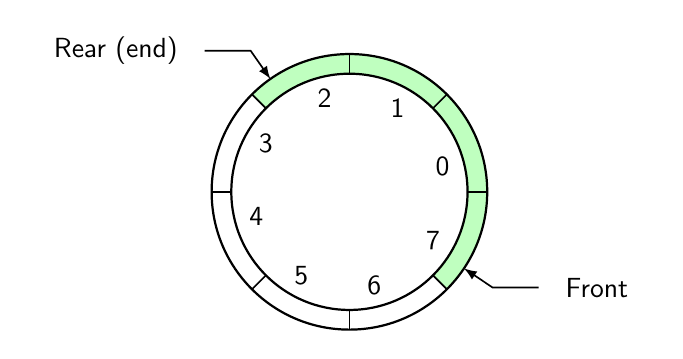
\begin{tikzpicture}[>=latex,font=\sffamily,semithick,scale=1.75]
		\fill [green!25] (0,0) -- (135:1) arc [end angle=-45, start angle=135, radius=1] -- cycle;
		\draw [thick] (0,0) circle (1);
		\foreach \angle in {90,45,...,-45}
			 	\draw (\angle:1) -- (\angle-180:1);
		\node [circle,thick,fill=white,draw=black,align=center,minimum size=3cm] at (0,0) {};
		\draw [<-] (125:1) -- (125:1.25) -- +(-.333,0)
			node [left,inner xsep=.333cm] (Head) {Rear (end)};
		\draw [<-] (-33.75:1) -- (-33.75:1.25) -- +(.333,0)
			node [right,inner xsep=.333cm] (Tail) {Front};(Head.west);
		
		\path 
		(15 :.7cm) node[]{0}
		(60 :.7cm) node[]{1}
		(105:.7cm) node[]{2}
		(150:.7cm) node[]{3}
		(195:.7cm) node[]{4}
		(240:.7cm) node[]{5}
		(285:.7cm) node[]{6}
		(330:.7cm) node[]{7};
\end{tikzpicture}
\end{center}
\end{frame}

\begin{frame}{Performance of Circular Array}
We assume a circular array with \textbf{fixed} size and both front and rear pointer. 

\vspace{-.1in}
\begin{table}
	\begin{tabular}{l | c | l }
		Operation & Performance & Note \\
		\hline \hline
		Insert at front & Super fast  & \\ 
		Deletion at front & Super fast & Move front ptr\\
		Insert at end & Super fast & \\
		Deletion at end & Super fast & Move rear ptr\\
		Insert at middle & Reasonable & How?\\
		Deletion at middle & Reasonable & How?\\
		Random access & Super fast & How?\\
		Forward iteration & Easy & \\
		Backward iteration & Easy & \\
		Memory consumption & Least & Unused space \\
	\end{tabular}
\end{table}
\end{frame}

\begin{frame}{A note on the performance}

\end{frame}	

\subsection{Standard Template Library}
\begin{frame}{History of the standard template library}

\end{frame}

\begin{frame}{\texttt{std::vector}}

\end{frame}

\begin{frame}{\texttt{std::list}}

\end{frame}

\begin{frame}{\texttt{std::map}}

\end{frame}

\begin{frame}{\texttt{std::unordered\_map}}

\end{frame}